

\chapter{Sistema de informação: análise de requisitos e arquitetura}






\section{Análise de requisitos}





\subsection{Requisitos funcionais}


%Os requisitos funcionais especificam os critérios que devem ser usados ​​para avaliar comportamentos ou funções especificas do sistema. Estes são os requisitos funcionais propostos no contexto deste projeto. 





\subsubsection{Dashboard}


\begin{itemize}
	\item A interface do sistema deve permitir que o utilizador, seja ele qual for, entre ou faça \textit{login} no sistema. 
	
	\item A interface do sistema deve permitir que o utilizador, seja ele qual for, saia ou faça \textit{logout} no sistema.
	
	\item O dashboard deverá permitir que qualquer utilizador possa recuperar a sua chave de acesso ao sistema.
	
	\item O sistema deve permitir que qualquer utilizador se possa registar no sistema, embora tenha que estar obrigatoriamente associado a uma empresa.
	
	\item O utilizador comum só terá acesso à sua área reserva após a validação por parte da empresa.   
	
	\item O dashboard deverá permitir ao administrador a adição de novas empresas e a gestão de todos os utilizadores. 
	
	\item O sistema deve permitir que qualquer utilizador possa adicionar, editar ou remover: 
	\begin{itemize}
		\item Tipos de sensores 
		\item Tipos de comunicação 
		\item Controller modules
		\item Tipo de comunicação a um controller modudel
		\item Sensor modules a um determinado Controller modules
		\item Um ou vários tipos de comunicação de um Sensor moduel
		\item Um ou vários sensores a um sensor moduel em que cada sensor é de um determinado tipo 
		
	\end{itemize}
	
	\item Visualizar graficamente os dados de cada sensor para um determinado \ac{SM}. 
	
	
	\item Visualizar em modo tabular os dados de cada sensor para um determinado \ac{SM}. 
	
	\item Em cada uma das visualizações anteriormente descritas, pretende-se que seja possível filtrar efetuar uma filtragem por data
	
	
	\item O sistema permitirá a exportação dos dados de uma determinado \ac{SM} em formato \ac{CSV}. 
	
	
	
	\item O sistema deve permitir o armazenamento de informações do cliente.
	
	\item O sistema deve permitir a atualização das informações do cliente.
\end{itemize}


\subsubsection{Aplicação mobile}



\begin{itemize}
	\item A interface da aplicação mobile deve permitir que o utilizador, seja ele qual for, entre ou faça \textit{login} no sistema. 
	
	\item A interface da aplicação mobile deve permitir que o utilizador, seja ele qual for, saia ou faça \textit{logout} no sistema.
	
	
	\item Visualizar graficamente os dados de cada sensor para um determinado \ac{SM}. 
	
	\item Receber alarmes quando um determinado valor lido está fora do estipulado.
	
	
\end{itemize}



\subsection{Requisitos não funcionais}


Requisitos não funcionais são todos os requisitos da aplicação relacionados com
performance, escalabilidade, segurança, disponibilidade e usabilidade. Estes não são
necessariamente pedidos pelo cliente. 


\begin{itemize}
	\item O sistema deverá executar em qualquer plataforma.
	
	\item O sistema deverá disponibilizar uma API para que possam ser criados novos produtos com base neste 
 
	
\end{itemize}








\subsection{Entidades envolventes}


No contexto deste sistema existem três entidades distintas que são importantes numerar: 

\begin{itemize}
	
	\item \textbf{General user}: este poderá registar-se e associando-se a uma determinada empresa registada no sistema. Após a validação por parte da empresa este utilizador poderá aceder à sua área reservada através das dashboard ou aplicação mobile. 
	
	\item \textbf{Companny user}: utilizador que gere todos os general users que se possam associar a si. Deste modo, este utilizador poderá validar os general users que a si se associam ou eliminá-los caso a permissão não seja desejada.  
	
	\item \textbf{Administrador}: vulgarmente denominado por Admin. Pretende-se que apenas exista uma único administrador. Genericamente este utilizador tem a possibilidade de poder adicionar novas empresas ao sistema i.e. criar novas utilizador com permissões especificas. 
	
\end{itemize}



\newpage

\subsection{Casos de uso}


\begin{figure}[!htb]
	\centering
	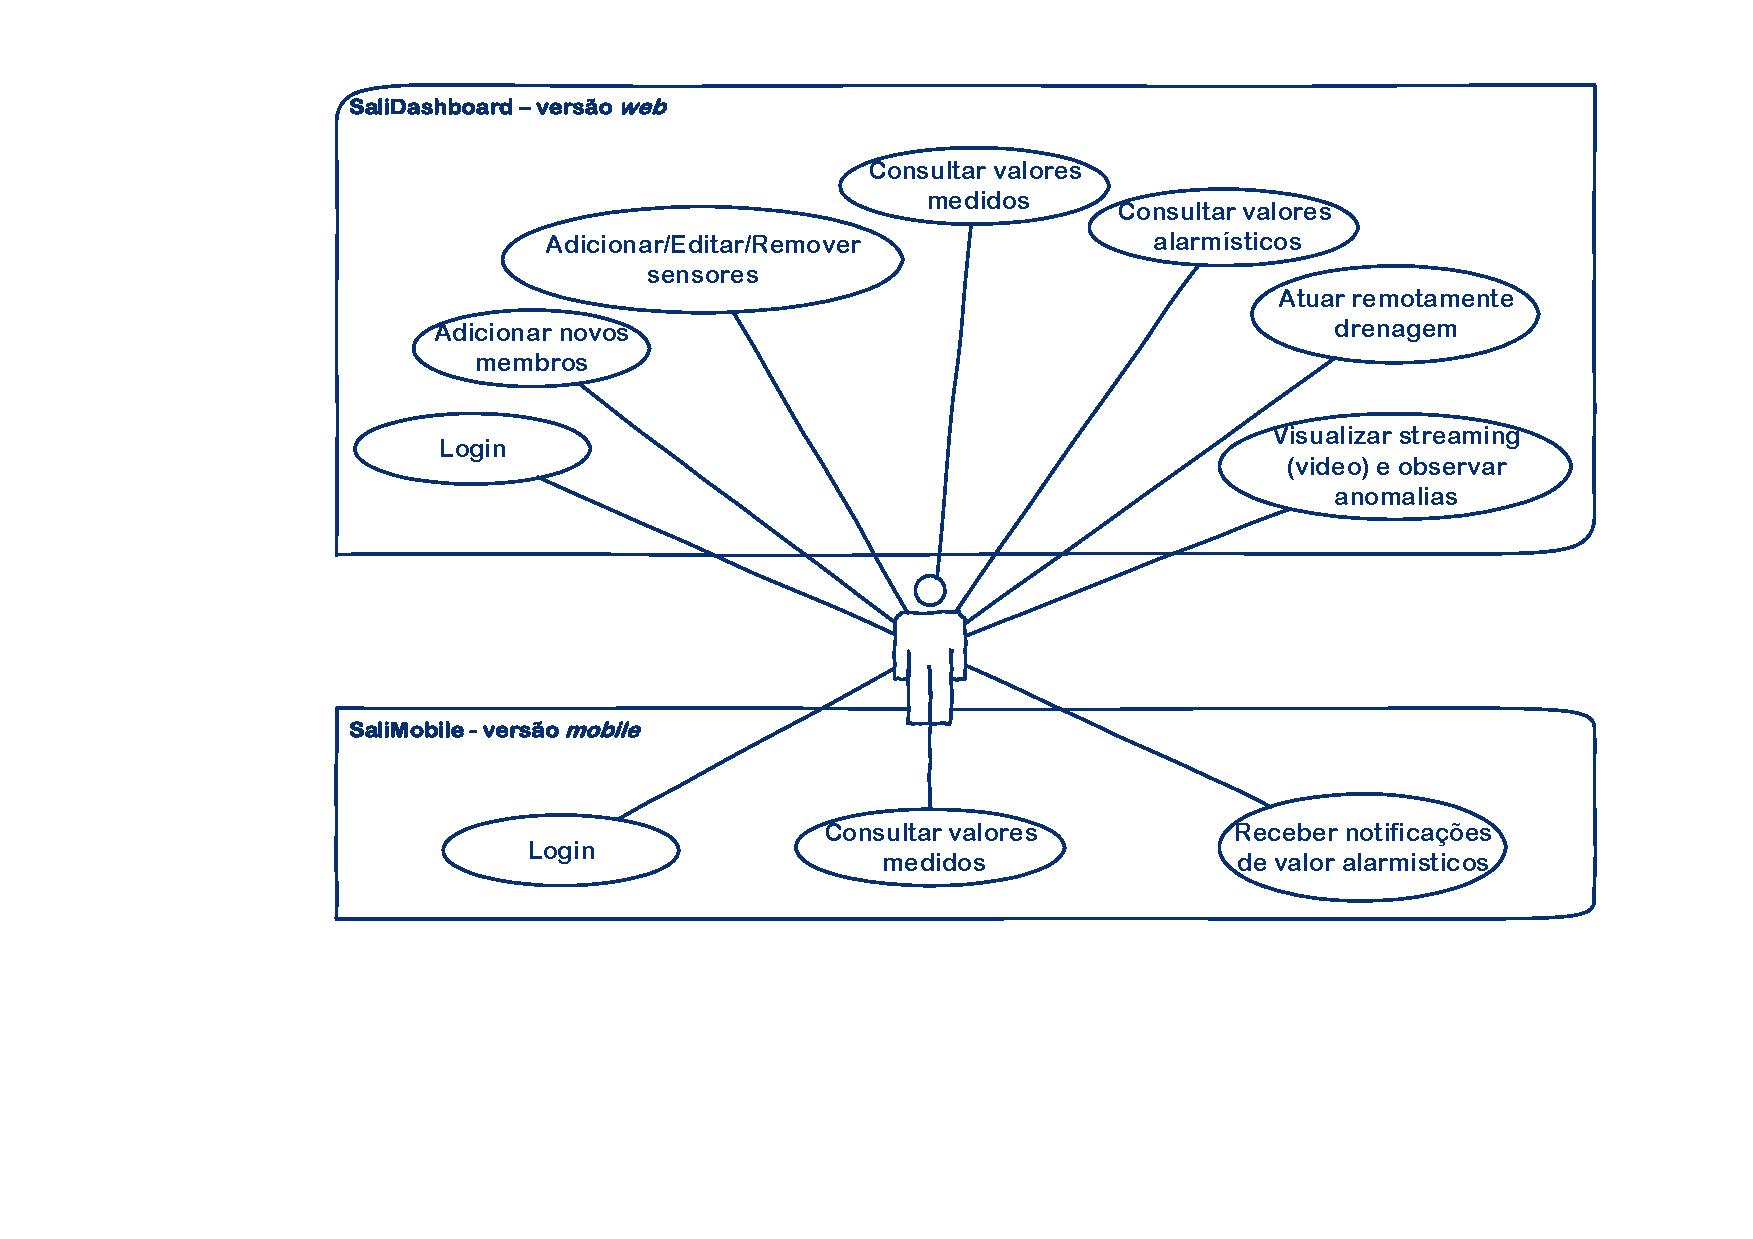
\includegraphics[scale=0.5]{esquemas/usecases.pdf}
	\caption{Pirâmide do conhecimento: modelo DIKW}
	\label{dikw}
\end{figure}











\newpage
\section{Modelo de dados}


\begin{figure}[!htb]
	\centering
	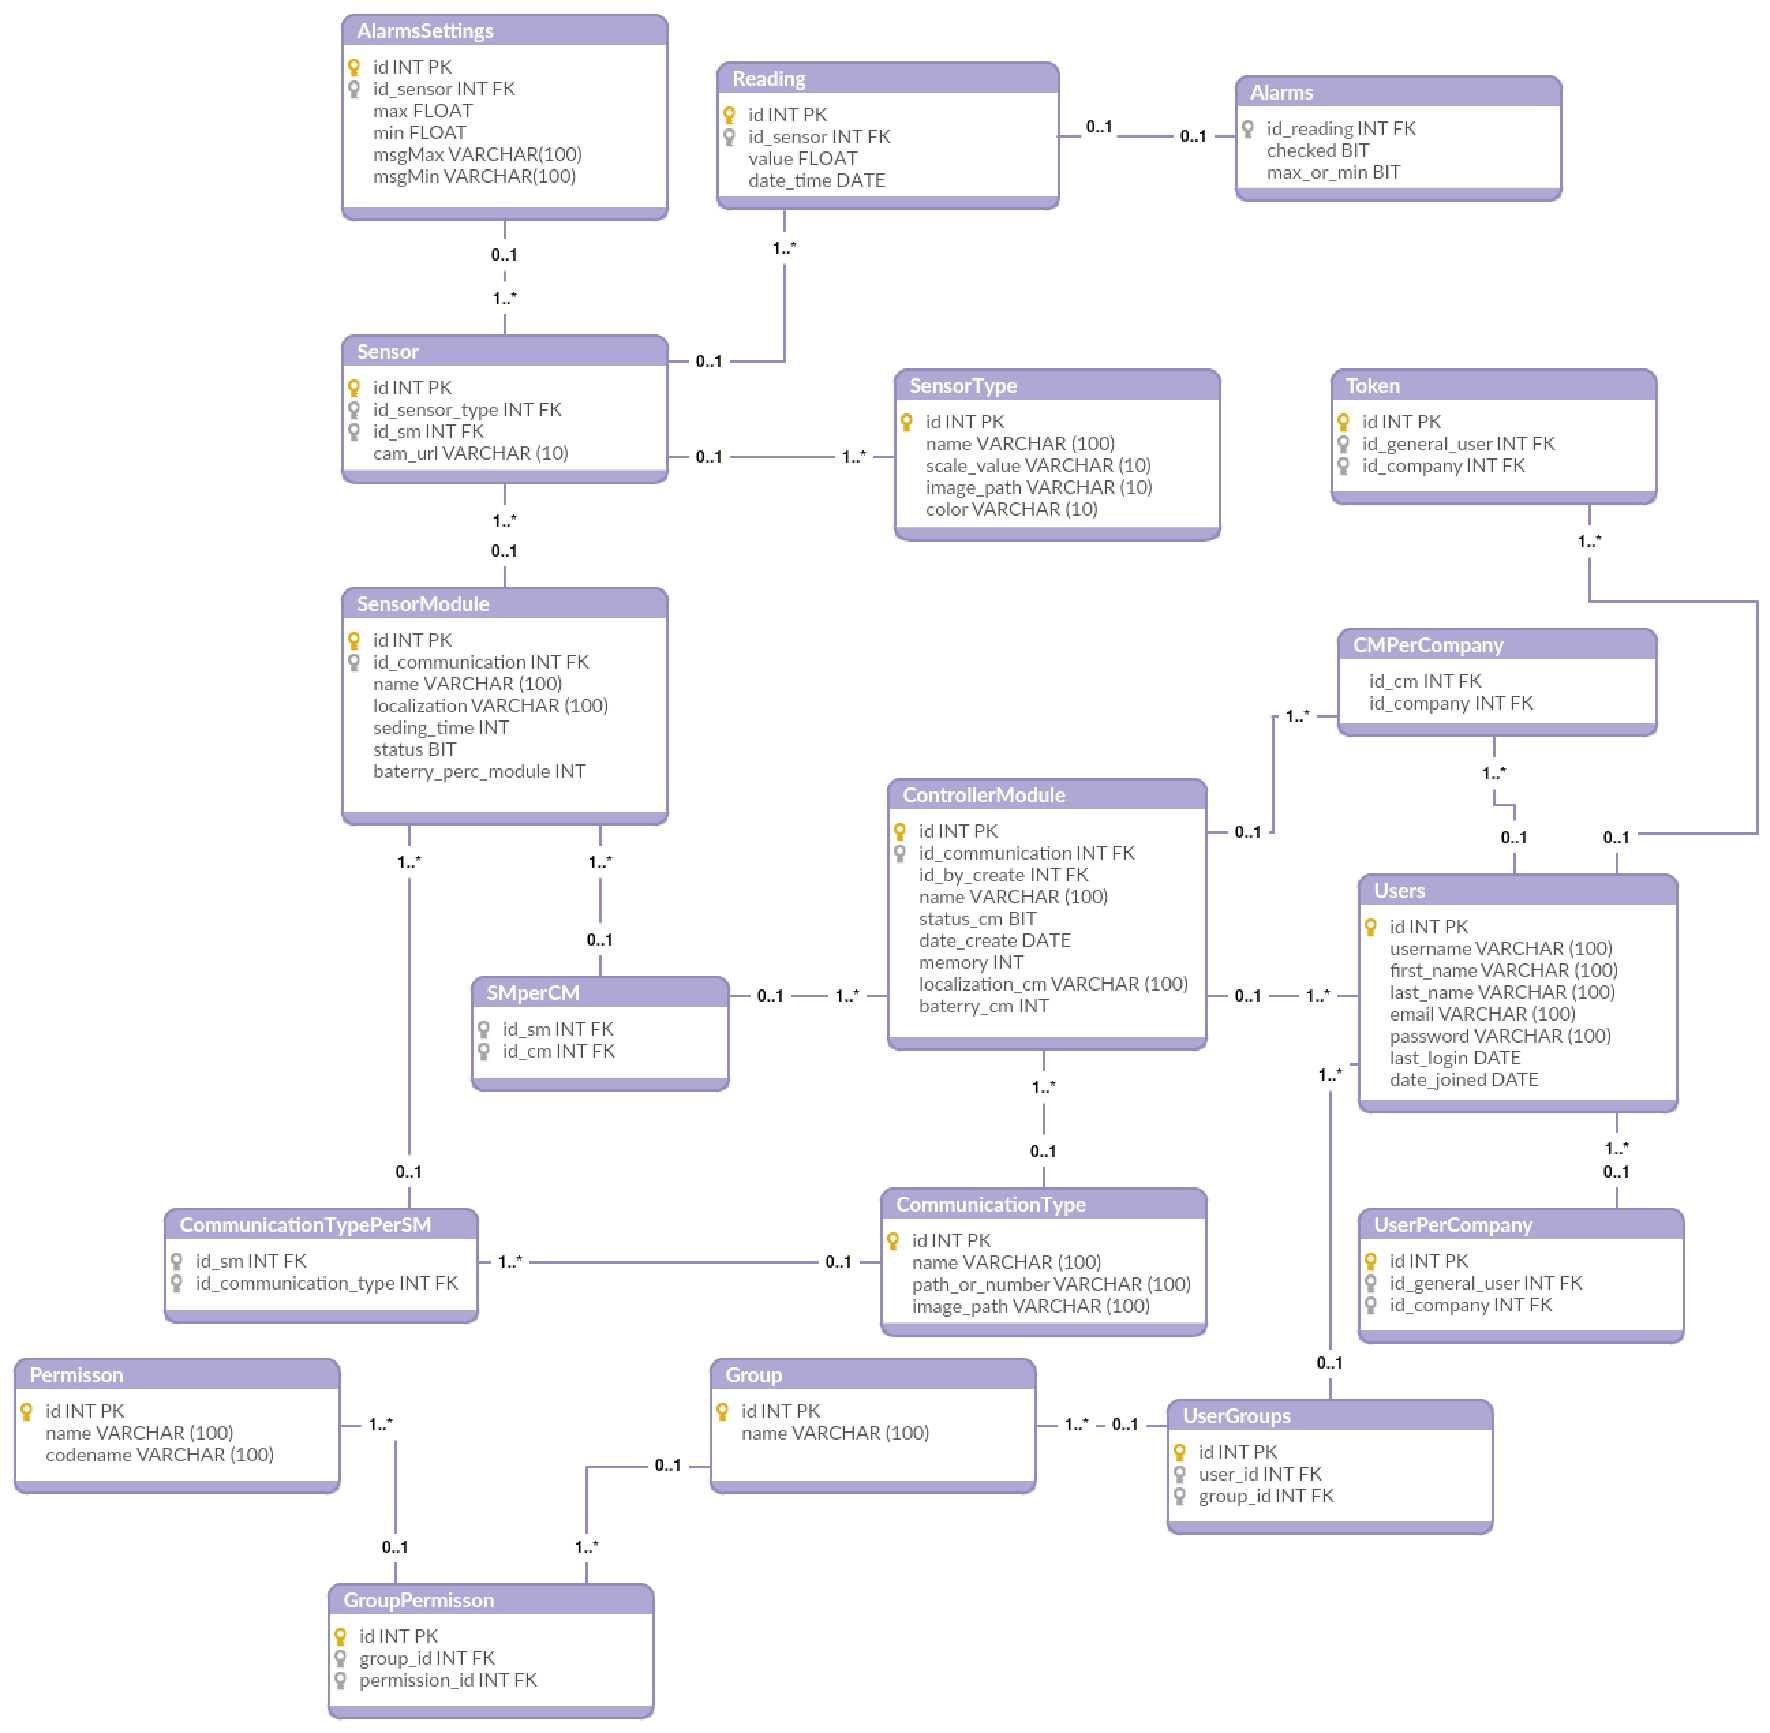
\includegraphics[scale=0.25]{esquemas/database_tese.pdf}
	\caption{Pirâmide do conhecimento: modelo DIKW}
	\label{db}
\end{figure}


\newpage

\begin{table}[h]
	\centering
	\begin{tabular}{|l|l|l|}
		\hline
		\multicolumn{1}{|c|}{\textbf{Nome}} & \multicolumn{1}{c|}{\textbf{Identificador}} & \multicolumn{1}{c|}{\textbf{Descrição}} \\ \hline
		User & auto-incrementado & dasdas \\ \hline
		ControllerModule&  &  \\ \hline
		SensorModule&  &  \\ \hline
		CommunicationType&  &  \\ \hline
		SensorType&  &  \\ \hline
		Sensor&  &  \\ \hline
		Reading&  &  \\ \hline
		AlarmsSettings&  &  \\ \hline
		Alarms&  &  \\ \hline
	\end{tabular}
	\caption{My caption}
	\label{my-label}
\end{table}









\newpage












\section{Design técnico}


\newpage
\section{Arquitetura lógica}



\begin{figure}[!htb]
	\centering
	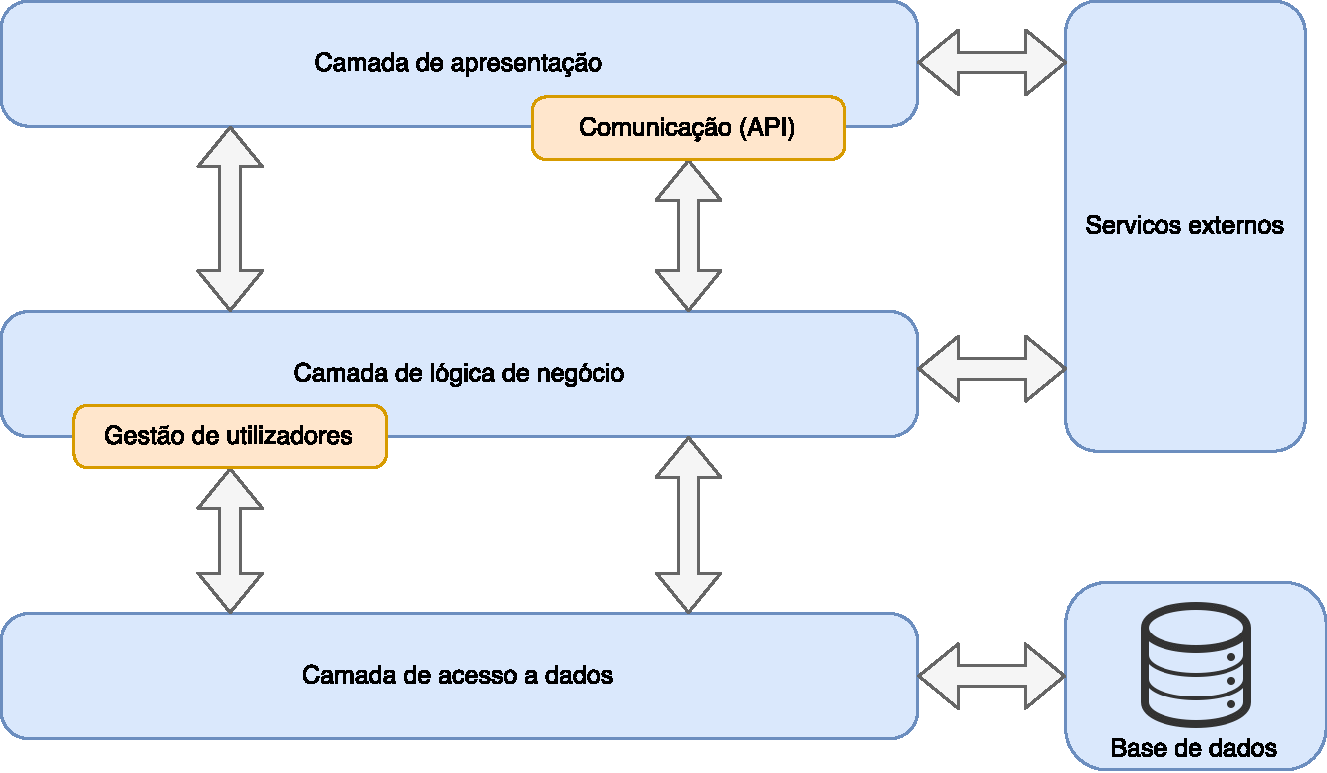
\includegraphics[width=\linewidth]{esquemas/arquitetura-logica.pdf}
	\caption{Arquitetura lógica}
	\label{opencvlogo}
\end{figure}



\subsection{Camada de apresentação}


A camada de apresentação é responsável pela comunicação entre os utilizadores e a aplicação, sendo ela web ou mobile, exibindo informações aos utilizadores, abrangendo uma interface que permite solicitações ao sistema.


A interface de usuário foi desenvolvida em HTML5 e CSS, fazendo uso de jQuery e Javascript.



\begin{itemize}
	\item \textbf{HTML5}: \ac{HTML} é a linguagem padrão usada para estruturar e apresentar conteúdo da web. HTML5 é a quinta versão do HTML.
	\item \textbf{CSS}: \ac{CSS} é uma linguagem usada para descrever a apresentação de conteúdo escrito em uma marcação Como HTML.
	\item \textbf{Javascript}: Javascript é a linguagem de programação para páginas da web.
	\item \textbf{JQuery}: JQuery é uma biblioteca Javascript que simplifica a programação Javascript
\end{itemize}









\subsection{Camada de lógica de negócio}



\subsection{Camada de acesso a dados}




\section{Arquitetura física}


\subsection{Sistema de informação}

\subsection{Aplicação web}


\subsection{Aplicação mobile}



%%%%%%%%%%%%%%%%%%%%%%%%%%%%%%%%%%%%%%%%%%%%%%%%%%%%%%%%%%


\section{Diagrama de componentes}




\section{Sistema de interação}


\section{Descrição}


Modulos da daniela : Cc1110



\section{Arquitetura geral}




\newpage









\section{Requisitos de funcionamento}


\newpage


\section{API}

Os métodos da API permitem executar as funções REST. Assim, torna-se fundamental perceber estes métodos para ter um melhor conhecimento do funcionamento do sistema. Como tal, de seguida, são descritos os métodos mais importantes que dão suporte a cada uma das funções REST.

\begin{itemize}
	\item \textbf{GET}: 
	\item \textbf{POST}: 
	\item \textbf{DELETE}: 
\end{itemize}





\begin{table}[h]
	\centering
	\begin{tabular}{|l|l|l|}
		\hline
		\multicolumn{1}{|c|}{\textbf{End point}} & \multicolumn{1}{c|}{\textbf{Tipo}} & \multicolumn{1}{c|}{\textbf{Descrição}} \\ \hline
		User & auto-incrementado & dasdas \\ \hline
		ControllerModule&  &  \\ \hline
		SensorModule&  &  \\ \hline
		CommunicationType&  &  \\ \hline
		SensorType&  &  \\ \hline
		Sensor&  &  \\ \hline
		Reading&  &  \\ \hline
		AlarmsSettings&  &  \\ \hline
		Alarms&  &  \\ \hline
	\end{tabular}
	\caption{My caption}
	\label{my-label}
\end{table}





\section{Valores simulados}



\section{\textit{Deploy} do projecto}


https://jee-appy.blogspot.com.tr/2015/04/deploy-django-project-on-apache-using.html

Caracteristicas da maquina virtual

Description:	Ubuntu 14.04.1 LTS
64 bitsRAM 2GB 

\section{Considerações finais}








